\section{Evaluation}

In this section we will evaluate our Guided Model selection approach by comparing the results with leaderboards of two forecasting competitions.


\subsection{M5 Forecast Accuracy Competition Results}


\begin{table}
\fontsize{9pt}{12pt}\selectfont
\begin{tabular}{rlllll|lp{5cm}}
\#      & $fh$ & Freq. & $sp$ & Strictly pos. & Window       & Model & Parameters \\
\hline
 27,616 &  28  & D     & 1    & no            & [4y,   100y) & Linear Regr. & deg: 1, deseasonal mod.: additive, fit intercept: yes, normalize: no, window: 56 \\
 13,191 &  28  & D     & 1    & no            & [480d, 4y)   & Linear Regr. & deg: 1, deseasonal mod.: additive, fit intercept: yes, normalize: no, window: 28 \\
 10,562 &  28  & D     & 7    & no            & [4y,   100y) & sNa\"ive     & sp: 7, strategy: mean, window: 112 \\
  7,976 &  28  & D     & 7    & no            & [480d, 4y)   & sNa\"ive     & sp: 7, strategy: mean, window: 112 \\
  1,107 &  28  & D     & 1    & no            & [180d, 480d) & Theta        & deseasonalize: no \\
    450 &  28  & D     & 7    & no            & [180d, 480d) & sNa\"ive     & sp: 7, strategy: mean, window: 28 \\     
     78 &  28  & D     & 1    & no            & [56d,  180d) & Theta        & deseasonalize: no
\end{tabular}
\caption{M5 competition: The evaluated models to be used per group of timeseries. The first column shows how many timeseries are in that group. Our approach seems to have chosen sNa\"ive for all timeseries that contain a weekly seasonality and Theta and Linear Regression for timeseries without seasonality. We also see that Theta is favored if the training window is shorter, vs Linear Regression that seems to perform better with longer windows.}
\label{tab:m5GroupsAndModels}
\end{table}


With our guided model selection approach and the gathered configuration summaries we can determine which models should work best for a new problem. To verify our approach, we tested it by running it for the M5 forecast competition dataset. We did not use the M5 dataset in our training, so we do not create a bias towards it. However, we have collected datasets that are similar in terms of sparsity, amplitude, length, and so forth. We particularly also had a sales data set from another competition in place besides others. So, there is a slight bias towards this kind of data in our training set.


\begin{figure*}
\centerline{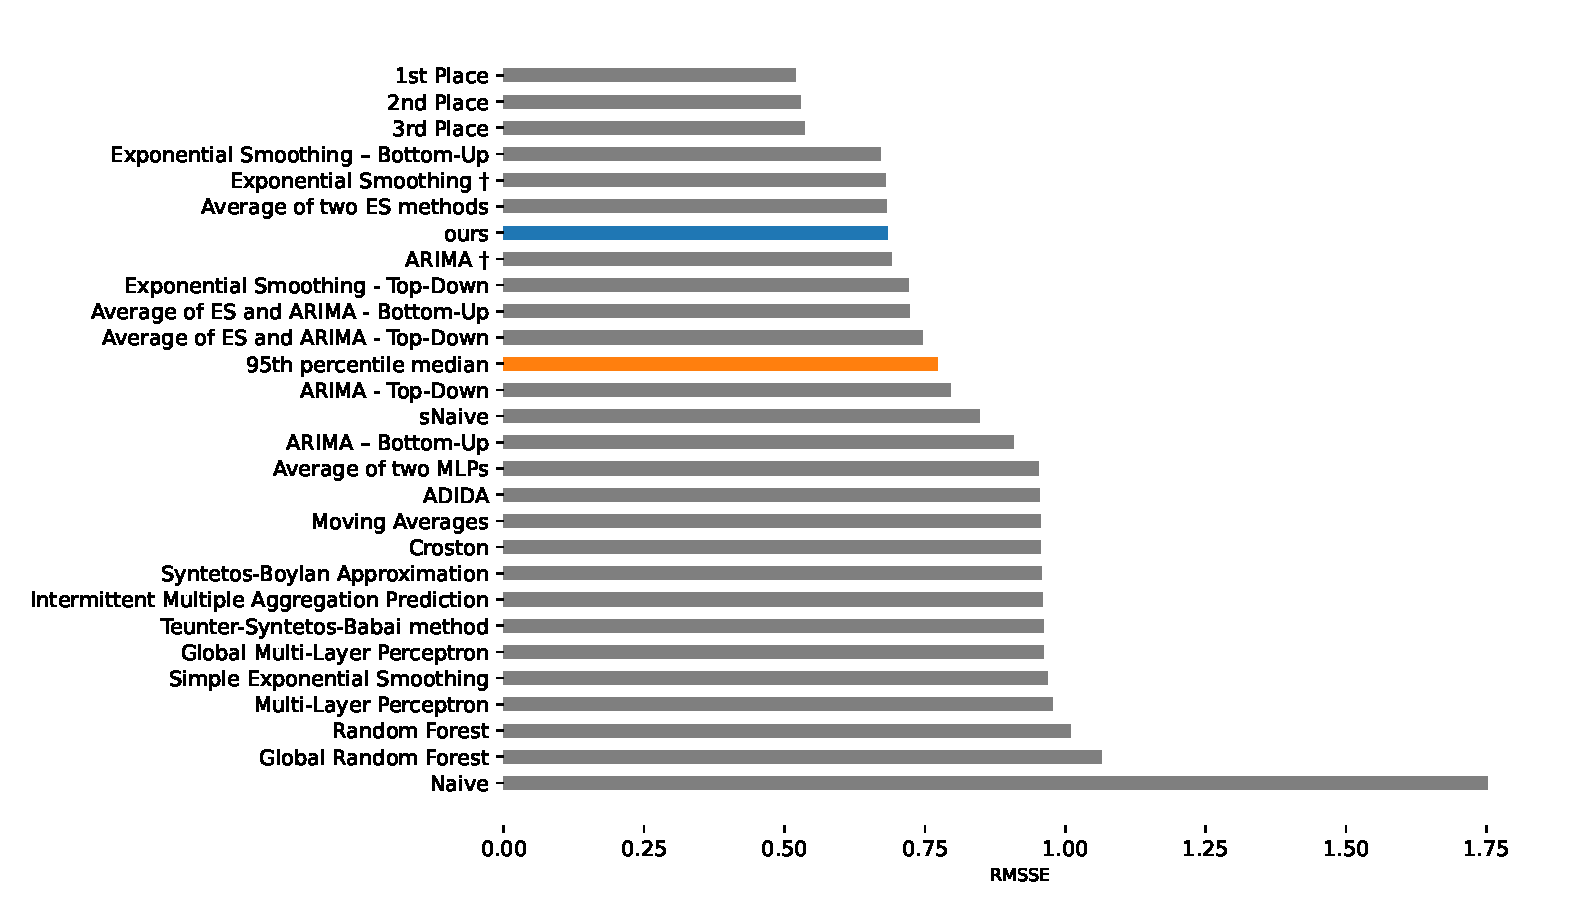
\includegraphics[scale=.6]{Figures/m5-leaderboard.eps}}
\caption{M5 Competition: The comparison of RMSSE scores with the top three places, ours and a series of baselines. \textdagger Model with explanatory (exogenous) variables. The 95\textsuperscript{th} percentile median is computed over all scores. We first took the percentile value and then built the median of all scores below that. Submitting forecasts with all zeros would result in a RMSSE score of 5.39065.}
\label{fig:m5-leaderboard}
\end{figure*}

First, we created the timeseries groups of the 30,490 M5 timeseries. This gave us the following set of groups and the best model for it. We only regard the accuracy metric as important for this competition, so we set the weights for CPU time and explainability to zero. See table \ref{tab:m5GroupsAndModels} for the elected models per group. The final submission is a combination of both validation and evaluation timeseries, which is why the total number of timeseries per group is doubled in this table.

We then created forecasts with those models and uploaded it to Kaggle. On Kaggle there usually are two leaderboards. For the M5 competition the public leaderboard is based on validation data that has been provided during the competition timeframe. Thus, it is possible to cheat and use the provided data to train a forecaster. The private leaderboard is based on hidden test data and each forecast's RMSSE score is weighted per timeseries with unknown weights. The leaderboards are calculated with approximately 50\% of the test data. Figure \ref{fig:m5-leaderboard} shows the leaderboard with the top three participants, our approach and a series of benchmarks. The benchmark scores are based on the results published by the hosts of the M5 competition. We have reproduced the Na\"ive and sNa\"ive scores and ended up with numerically almost the same scores.

Our approach resulted in a RMSSE score of 0.68382. This score is in the top 8.8\% of all submissions. We find that score to be competitive as only one single model benchmark had a lower error term. We would not expect to have a significantly lower error than the best benchmarks since we are only using benchmark models ourselves, although in a combined fashion. We also computed the forecast in less time than most of those benchmark models take by themselves since we had 31\% of our timeseries forecasted with sNa\"ive, a method that takes roughly 8ms to create a forecast. Linear Regression takes roughly 66ms and Theta 14ms. The total CPU time to compute the forecasts for the 60,980 timeseries was roughly 47 minutes. With multiprocessing on a machine with 8 cores, it took around 6 minutes (on a Macbook Pro, 2.6 GHz 6-Core Intel Core i7).

Although we do not know the times it took the competition hosts to compute the benchmark results, we argue that this ratio of accuracy and CPU time is hard to beat all the while did not even consider CPU time while selecting the models.

\subsection{Web Traffic Forecast Competition Results}

The Web Traffic Forecast competition requires participants to compute a 65-day forecast on roughly 145,000 timeseries. The forecast accuracy is measured in sMAPE, which is not ideal as we discussed earlier. The Web Traffic data is different from the M5 data in the sense that it contains a lot of strictly positive timeseries with high traffic values. We do not have a large amount of similar data in our datasets that we used to evaluate models. Specifically, we encountered that the largest group in the Web Traffic dataset had no equivalent dataset in our library to pick an evaluated model from. We used a fallback of sNa\"ive with strategy \emph{mean}. The groups designed to be generic also do not contain a forecasting horizon of 65 days. We took the closest value of 60 which likely had a small negative on finding the best models. The groups and mapped models can be seen in table \ref{tab:webTrafficGroupsAndModels}. Altogether, this proved to be not successful at all since our resulting sMAPE score was 61.08807. Our benchmarks for Na\"ive and sNa\"ive scored 49.26081 and 47.62652 respectively. The first three places reached scores of 35.48, 36.78 and 36.85. We find that valid and varied datasets are required to assume a well-fitting model can be recommended. Our models performed worse than a baseline method. We think this can also be attributed to the selection of Gradient Boosting which was chosen because of a bias towards less flaky data in our datasets than the web traffic data has.

We think we could improve this if we collect enough data and rerun our evaluation.

\begin{table}
\fontsize{9pt}{12pt}\selectfont
\begin{tabular}{rlllll|lp{5cm}}
\#      & $fh$ & Freq. & $sp$ & Strictly pos. & Window       & Model                & Parameters \\
\hline
 48,518 &  60  & D     & 7    & yes           & [480d,   4y) & Fallback to sNa\"ive & sp: 7, strategy: mean \\
 48.191 &  60  & D     & 1    & yes           & [480d,   4y) & Linear Regr.         & deg: 1, deseasonal mod.: add, fit~intercept: yes, normalize: yes, window: 60 \\
 42,460 &  60  & D     & 1    & no            & [480d,   4y) & Gradient Boosting    & deg: 1, deseasonal mod.: add, learn.~rate: 0.1, max~depth: 3, max~feat.: auto, n~estimators: 100, subsample: 1, sp: 1 \\
  5,892 &  60  & D     & 7    & no            & [480d,   4y) & Fallback to sNa\"ive & sp: 7, strategy: mean \\
      1 &  60  & D     & 1    & no            & [180d, 480d) & Theta                & deseasonalize: no \\
      1 &  60  & D     & 1    & no            & [0,     56d) & Fallback to sNa\"ive & sp: 7, strategy: mean \\
\end{tabular}
\caption{Web Traffic Competition: The evaluated models to be used per group of timeseries. Our missing data that contains weekly seasonality and is strictly positive required us to fallback to a baseline method for the biggest group.}
\label{tab:webTrafficGroupsAndModels}
\end{table}
